% =====================================================================
%  PRELIMINARY MANUSCRIPT  --  results pending
%  Fuzzy eye-tracking gating of EEG windows (M1) vs. hard-threshold gating (M0)
%  Generic article class: port to the target conference template
%  (Springer LNCS / IEEE conference) once it is known.
%  All result-dependent text is marked with \pending{...} or \revise{...}.
% =====================================================================
\documentclass[11pt,a4paper]{article}
\usepackage[T1]{fontenc}
\usepackage[utf8]{inputenc}
\usepackage{lmodern}
\usepackage[margin=2.3cm]{geometry}
\usepackage{amsmath,amssymb,bm}
\usepackage{graphicx}
\usepackage{booktabs,multirow,tabularx,array}
\usepackage{xcolor}
\usepackage{algorithm}
\usepackage{algpseudocode}
\usepackage{tikz}
\usetikzlibrary{positioning,arrows.meta,fit,backgrounds,calc}
\usepackage[hidelinks]{hyperref}
\usepackage{caption}
\captionsetup{font=small,labelfont=bf,labelsep=space}

% ---------- placeholder macros (search for "PENDING" / "REVISE") ----------
\newcommand{\pending}[1]{\textcolor{red!75!black}{\textbf{[PENDING: #1]}}}
\newcommand{\revise}[1]{\textcolor{orange!80!black}{\textit{[REVISE AFTER RESULTS: #1]}}}
\newcommand{\PND}{\textcolor{red!75!black}{\textbf{PENDING}}}
\newcommand{\dataset}{ZuCo~1.0}

\title{Fuzzy Eye-Tracking Gating of EEG Windows for Affective State Classification:\\
An Experimental Comparison with Hard-Threshold Gating in a Sugeno Fuzzy Rule-Mining Framework}
\author{\pending{Author names and affiliations}}
\date{\pending{Preliminary draft --- 4 November 2026}}

\begin{document}
\maketitle

% =====================================================================
\begin{abstract}
\noindent
Multimodal emotion recognition from electroencephalography (EEG) commonly assumes that the label attached to a stimulus holds for its entire duration, although the affective response evoked by a stimulus is neither constant nor uniformly timed. A recent approach addresses this assumption by using an eye-tracking feature, the mean pupil diameter, as a hard gate: only EEG segments at which the feature reaches a threshold are retained, and the retained segments are described by wavelet-band entropy features and classified with genetic-algorithm-tuned Sugeno fuzzy rules. A hard gate, however, discards every sub-threshold segment, responds abruptly to small fluctuations around the threshold, and treats a noisy and luminance-sensitive ocular measurement as a reliable binary indicator. This paper investigates whether replacing the hard gate with a fuzzy gate is a more flexible alternative. In the proposed model, the same normalised eye-tracking feature is partitioned into Low, Medium and High fuzzy sets, and a zero-order Sugeno rule base maps the memberships to a continuous relevance weight in $[0,1]$ for every EEG window. The weights modulate the contribution of each window both during fuzzy rule mining and during trial-level aggregation of window decisions, while the EEG preprocessing, discrete wavelet decomposition, entropy features, minimum-redundancy-maximum-relevance feature selection and Sugeno classifier of the baseline are kept unchanged. The hard gate is recovered as a limiting case of the fuzzy gate, so the comparison isolates the effect of the gating function. Both models are evaluated on the publicly available \dataset{} corpus of simultaneous EEG and eye-tracking recordings \pending{confirm final dataset} under subject- and stimulus-disjoint cross-validation designed to prevent window-level data leakage. \revise{Insert baseline and proposed accuracy, macro-F1 and the outcome of the paired statistical test; state whether fuzzy gating improved, matched or degraded performance.}
\end{abstract}

\noindent\textbf{Keywords} Electroencephalogram (EEG) $\cdot$ Eye tracking $\cdot$ Emotion recognition $\cdot$ Fuzzy gating $\cdot$ Sugeno fuzzy inference system $\cdot$ Multimodal fusion

% =====================================================================
\section{Introduction}
\label{sec:intro}

Automatic recognition of human affective states supports applications in mental-health assessment, adaptive human--computer interaction and user-experience evaluation. Among the physiological signals used for this purpose, the electroencephalogram (EEG) is attractive because it records cortical activity non-invasively with millisecond temporal resolution and at a cost far below that of functional neuroimaging \cite{Alarcao2019,Jenke2014}. EEG-based emotion recognition has progressed from band-power features with conventional classifiers to entropy-based and deep representations, and accuracies above 80\% are routinely reported on benchmark corpora such as DEAP, MAHNOB-HCI and the SEED family \cite{Koelstra2012,Soleymani2012db,ZhengLu2015,Zheng2019}.

Eye tracking provides a complementary, low-cost view of the same affective process. Pupil diameter increases with emotional arousal irrespective of valence \cite{Bradley2008,Partala2003}, and fixation and saccade statistics reflect the allocation of attention to a stimulus \cite{Lim2020}. Several studies have shown that fusing EEG with eye-movement features improves recognition accuracy over either modality alone, for example from 78.51\% (EEG) and 77.80\% (eye movements) to 87.59\% with fuzzy-integral decision fusion \cite{Lu2015}, and to 85.11\% for four emotions on SEED-IV with multimodal deep learning \cite{Zheng2019}.

A less frequently addressed problem is the \emph{temporal validity of labels}. Emotion corpora assign one label to an entire stimulus, yet there is no guarantee that the intended emotion is present throughout the stimulus or that it is elicited at a predictable moment. When a long recording is cut into short windows that all inherit the stimulus label, many windows carry little or no affective information, which corrupts both training and evaluation. Farhadi Sedehi et al.\ \cite{FarhadiSedehi2024a} proposed to use eye tracking as a \emph{gate} for this purpose. Eight eye-tracking features are ranked with minimum-redundancy-maximum-relevance (mRMR) selection; the highest-ranked feature, the mean pupil diameter in the vertical direction, is compared with a threshold, and only EEG segments at the corresponding moments are processed. The selected segments are decomposed into five frequency bands with the discrete wavelet transform (DWT), four entropy measures are extracted, three features are selected with mRMR, and a Sugeno fuzzy inference system (S-FIS) whose rules are refined by a genetic algorithm (GA) assigns one of four emotional categories. The authors reported 94.42\% and 85.20\% average accuracy in the alpha band on SEED-IV and MAHNOB-HCI, respectively \cite{FarhadiSedehi2024a}, and later reused pupil-based gating in a Granger-causality model \cite{FarhadiSedehi2024b}.

The gating idea is appealing, but its hard-threshold form has properties that motivate further investigation. First, the gate is binary: a window whose pupil feature lies marginally below the threshold is discarded completely, whereas one marginally above it is retained with full weight, so small measurement fluctuations can change the training set and the evidence available at test time. Second, pupil diameter is dominated by the pupillary light reflex and is also modulated by cognitive load, gaze position and tracking quality \cite{Mathot2018,Raiturkar2016,Holmqvist2012}; treating a single threshold crossing as a certain indicator of affective relevance ignores this uncertainty. Third, discarding windows reduces the amount of EEG evidence and may leave some trials with very few or no windows. Fuzzy set theory \cite{Zadeh1965} offers a natural way to express graded relevance: instead of declaring a window relevant or irrelevant, a membership function can express the degree to which its eye-tracking evidence indicates affective engagement. Soft gating has a long history in machine learning \cite{Jacobs1991,Arevalo2020}, and fuzzy membership has been used to weight individual training samples \cite{LinWang2002}. However, to the best of our knowledge, it has not been used to weight EEG time windows from eye-tracking evidence for emotion recognition.

This paper therefore asks the following research question: \emph{Does a fuzzy eye-tracking gate, which assigns each EEG window a continuous relevance weight, provide a more flexible and effective alternative to hard-threshold gating within an otherwise unchanged fuzzy rule-mining emotion-recognition pipeline?} The question is posed as a hypothesis to be tested; it is not assumed that the fuzzy gate improves accuracy.

\subsection{Motivation}
The motivation is threefold. (i) Graded relevance is a more faithful representation of an uncertain ocular indicator than a crisp threshold. (ii) A fuzzy gate retains every window, so no trial is left without evidence and the training set does not change discontinuously with the threshold. (iii) Because the baseline classifier is itself a fuzzy rule base, a fuzzy gate keeps the whole pipeline interpretable: each weight can be traced to linguistic rules such as ``if the pupil feature is High, then the window is highly relevant''.

\subsection{Contributions}
The contributions of this paper are as follows.
\begin{enumerate}
  \item We formalise the hard eye-tracking gate of \cite{FarhadiSedehi2024a} as a crisp window-weighting function and re-implement the baseline pipeline (M0) on a publicly available simultaneous EEG and eye-tracking corpus, documenting every implementation decision that the original description leaves open.
  \item We propose a fuzzy gate (M1) in which the same eye-tracking feature is fuzzified into Low, Medium and High sets and mapped by a zero-order Sugeno rule base to a continuous window weight. The hard gate is a limiting case of the fuzzy gate, so M0 and M1 differ in exactly one component.
  \item We integrate the window weights at two points of the S-FIS-GA pipeline: as sample weights in rule mining and GA fitness evaluation, and as aggregation weights when window-level decisions are combined into a trial-level prediction.
  \item We compare M0 and M1 under subject- and stimulus-disjoint cross-validation in which all data-dependent steps are fitted on training folds only, and we report class-wise metrics, confusion matrices, paired statistical tests and computational cost. \revise{Summarise the empirical finding in one sentence.}
\end{enumerate}

\subsection{Organization of the paper}
Section~\ref{sec:related} reviews related work and Sect.~\ref{sec:gap} states the research gap. Section~\ref{sec:method} describes the baseline and the proposed fuzzy-gating model. Section~\ref{sec:data} describes the dataset and Sect.~\ref{sec:setup} the experimental protocol. Section~\ref{sec:results} presents the results and discussion, Sect.~\ref{sec:limits} the limitations, and Sect.~\ref{sec:conclusion} concludes the paper. Table~\ref{tab:abbr} lists the abbreviations used throughout.

\begin{table}[t]
\centering\small
\caption{List of abbreviations}\label{tab:abbr}
\begin{tabular}{@{}ll@{\hspace{2em}}ll@{}}
\toprule
Abbreviation & Description & Abbreviation & Description\\
\midrule
EEG & Electroencephalogram & mRMR & Min.-redundancy max.-relevance\\
ET & Eye tracking & S-FIS & Sugeno fuzzy inference system\\
DWT & Discrete wavelet transform & GA & Genetic algorithm\\
SampEn & Sample entropy & MF & Membership function\\
PermEn & Permutation entropy & LOSO & Leave-one-subject-out\\
SymbEn & Symbolic dynamics entropy & CV & Cross-validation\\
PhEn & Phase entropy & SR & Sentiment reading (ZuCo task)\\
M0 & Hard-gated baseline model & M1 & Proposed fuzzy-gated model\\
\bottomrule
\end{tabular}
\end{table}

% =====================================================================
\section{Related works}
\label{sec:related}

\subsection{EEG-based emotion recognition}
EEG emotion recognition pipelines typically consist of artefact removal, segmentation, feature extraction, feature selection and classification \cite{Alarcao2019}. Frequency-domain features remain dominant. Duan et al.\ \cite{Duan2013} introduced differential entropy (DE) and reported 84.22\% accuracy against 76.56\% for the energy spectrum, and Zheng and Lu \cite{ZhengLu2015} used deep belief networks on DE features of the SEED dataset to identify critical frequency bands and channels, obtaining 86.08\% average accuracy with comparable performance from reduced 4--12 channel montages. Time--frequency decomposition with the DWT is a common alternative to Fourier analysis because it provides band-limited sub-signals with good temporal localisation; Murugappan et al.\ \cite{Murugappan2010} used Daubechies-4 wavelets to extract alpha, beta and gamma components and reached 83.26\% with a k-nearest-neighbour classifier on five discrete emotions. Nonlinear complexity measures such as sample entropy \cite{Richman2000}, permutation entropy \cite{Bandt2002}, symbolic dynamics entropy \cite{Zebrowski2000} and phase entropy \cite{Rohila2019} have been adopted because EEG is non-stationary and nonlinear. Jenke et al.\ \cite{Jenke2014} compared features from 33 studies and found that such advanced features outperformed plain band power and that multivariate feature selection performed slightly better than univariate selection. The mRMR criterion \cite{Peng2005} is a widely used multivariate filter that selects features with high mutual information with the class and low mutual information with one another.

A recurring concern in this literature is evaluation validity. Li et al.\ \cite{Li2021} demonstrated that block-designed EEG experiments, in which training and test samples originate from the same continuous recording block, allow classifiers to exploit temporal correlations unrelated to the stimulus class. For emotion recognition, a review of 101 DEAP studies reported that segmentation leakage, feature selection on the full dataset and related errors were common and could inflate accuracy substantially \cite{Khan2025}, and a review of 216 papers reported inconsistent splitting and metrics across the field \cite{Kukhilava2025}. Both reviews are preprints and are cited here as indicative evidence. The cross-session drop reported for SEED-IV, from 85.11\% within sessions to 72.39\% across sessions \cite{Zheng2019}, further illustrates how strongly the evaluation protocol affects reported performance.

\subsection{Eye tracking and emotion}
The pupil dilates in response to emotionally arousing pictures and sounds, both pleasant and unpleasant, and this dilation co-varies with skin conductance, indicating sympathetic activation \cite{Bradley2008,Partala2003}. Pupil size therefore indexes arousal rather than valence. It is also governed primarily by the light and near responses, of which the psychosensory component is comparatively small \cite{Mathot2018}. For dynamic stimuli such as films, luminance changes must be modelled or removed before pupil size can be interpreted as arousal \cite{Raiturkar2016}, and Lu et al.\ explicitly removed the light reflex before using pupil features for emotion recognition \cite{Lu2015}. Pupil and gaze data further suffer from blinks, data loss and limited precision, which must be measured and reported \cite{Holmqvist2012}; standard preprocessing guidelines address blink removal, interpolation and smoothing \cite{Kret2019}. Lim et al.\ \cite{Lim2020} surveyed eye-tracking emotion recognition and identified pupil diameter, fixation, saccade and blink features as the most commonly used, while noting that eye tracking alone remains a relatively immature approach.

\subsection{Multimodal EEG and eye-tracking emotion recognition}
Zheng et al.\ \cite{ZhengDong2014} combined EEG with pupil-diameter features from five subjects watching film clips and obtained 71.77\% (EEG), 58.90\% (eye tracking) and 73.59\% (feature-level fusion) for three classes. Soleymani et al.\ \cite{Soleymani2012mm} fused EEG with pupil response and gaze distance at decision level and, under a participant-independent protocol, reached 68.5\% and 76.4\% for three-class valence and arousal, respectively. Lu et al.\ \cite{Lu2015} compared feature-level, decision-level and fuzzy-integral fusion of 16 eye-movement features with EEG; the fuzzy integral, which combines classifier outputs according to the importance of each source \cite{ChoKim1995}, produced the best accuracy of 87.59\%. EmotionMeter \cite{Zheng2019} introduced the four-class SEED-IV dataset and showed that EEG and eye movements are complementary: EEG recognised happiness better, whereas eye movements recognised fear better. Liu et al.\ \cite{Liu2022} compared deep canonical correlation analysis and bimodal autoencoders across five datasets, adding weighted-sum and attention-based fusion, and achieved 87.5\% on SEED-IV. Fu et al.\ \cite{Fu2023} aligned 4-s EEG and eye-movement windows in a two-branch network with multi-scale attention fusion and reported 87.32\% on SEED-IV.

In all of these studies the eye-tracking signal is a source of \emph{features} or \emph{decisions} to be fused with EEG. The gated approach of Farhadi Sedehi et al.\ \cite{FarhadiSedehi2024a,FarhadiSedehi2024b} is different in kind: eye tracking determines \emph{which EEG segments} are analysed, so it acts as a temporal selector rather than as a feature source. Table~\ref{tab:related} summarises the reviewed multimodal studies. Accuracies are copied from the original papers and are not directly comparable, because datasets, class definitions and validation protocols differ.

\begin{table}[t]
\centering\scriptsize
\caption{Summary of related EEG and eye-tracking emotion-recognition studies (results as reported by the original authors)}\label{tab:related}
\begin{tabularx}{\linewidth}{@{}p{0.9cm}p{1.5cm}p{3.0cm}p{2.0cm}p{1.6cm}X@{}}
\toprule
Ref. & Dataset & Method & Use of eye tracking & Result & Limitation\\
\midrule
\cite{ZhengDong2014} & Own (5 subj., 3 cl.) & PSD/DE, SVM, FLF/DLF & Pupil features fused & 73.59\% & Very small sample$^\dagger$\\
\cite{Soleymani2012mm} & MAHNOB proto. (24 subj.) & EEG + pupil/gaze, DLF & Features fused & 68.5\% V, 76.4\% A & Trial-level only; no temporal selection$^\ast$\\
\cite{Lu2015} & SEED-style (9 subj., 3 cl.) & DE + 16 eye features, fuzzy integral & Features + fuzzy DLF & 87.59\% & Within-session; fusion at output level$^\ast$\\
\cite{Zheng2019} & SEED-IV (4 cl.) & DE/PSD, multimodal DNN & Features fused & 85.11\% & Cross-session drop to 72.39\%\\
\cite{Liu2022} & SEED, SEED-IV, SEED-V, DEAP, DREAMER & DCCA/BDAE, attention fusion & Features fused & 87.5\% (SEED-IV) & Learned modality weights, not per window$^\ast$\\
\cite{Fu2023} & SEED-IV & Two-branch net, multi-scale attention & Features fused & 87.32\% & Black-box; weights not temporal$^\ast$\\
\cite{FarhadiSedehi2024a} & SEED-IV, MAHNOB-HCI (4 cl.) & DWT entropies, mRMR, S-FIS-GA & Hard pupil gate selects EEG segments & 94.42\%, 85.20\% & Segment-level 5-fold CV; crisp gate$^\ast$\\
\cite{FarhadiSedehi2024b} & MAHNOB-HCI (2 cl.) & Granger causality images, ResNet-18 & Hard pupil gate & 91.00\% & Crisp gate$^\ast$\\
\bottomrule
\multicolumn{6}{@{}l}{\scriptsize $^\dagger$ stated by the authors; $^\ast$ our analysis. FLF/DLF: feature-/decision-level fusion; V/A: valence/arousal.}
\end{tabularx}
\end{table}

\subsection{Fuzzy logic in emotion recognition and soft gating}
Fuzzy sets \cite{Zadeh1965} represent graded membership, and Takagi--Sugeno--Kang (TSK) models \cite{TakagiSugeno1985} combine fuzzy antecedents with functional or constant consequents. Rules can be generated from data with table look-up schemes such as that of Wang and Mendel \cite{WangMendel1992}, which is close to the look-up-table rule extraction used in the baseline, and membership parameters can be learned with neuro-fuzzy systems such as ANFIS \cite{Jang1993}. In emotion recognition, fuzzy rules have been used as interpretable EEG classifiers \cite{Matiko2014,FarhadiSedehi2024a}, fuzzy linguistic summaries have been applied to EEG time series \cite{Kaya2024}, and fuzzy integrals have fused EEG and eye-movement classifiers \cite{Lu2015,ChoKim1995}.

Gating, the use of one signal to modulate the contribution of another, has been studied separately. The mixture-of-experts model \cite{Jacobs1991} uses a soft gating network to weight expert outputs, and gated multimodal units learn multiplicative gates that decide how much each modality contributes \cite{Arevalo2020}. Classical classifier-combination theory analyses weighted sum and product rules \cite{Kittler1998}, and quality-aware fusion incorporates measured signal quality into score combination \cite{Nandakumar2008}. Fuzzy support vector machines assign each training sample a fuzzy membership that scales its influence on learning, reducing the effect of noisy samples \cite{LinWang2002}. These works establish soft weighting as an alternative to hard selection, but their weights are either learned and opaque, applied to modalities rather than time windows, or derived from the training sample itself rather than from a second modality.

% =====================================================================
\section{Research gap and contributions}
\label{sec:gap}

The literature leads to four observations. (a) EEG and eye-tracking fusion consistently improves on single modalities \cite{Lu2015,Zheng2019,Liu2022}, but eye tracking is almost always used as a feature source rather than as an indicator of \emph{when} EEG carries affective information. (b) The only approach we found that uses eye tracking for temporal selection of EEG \cite{FarhadiSedehi2024a,FarhadiSedehi2024b} applies a crisp threshold to a single pupil feature. (c) The ocular signal used for gating is uncertain: it reflects arousal rather than a specific emotion, is confounded by luminance, cognitive load and gaze geometry, and contains missing and noisy samples \cite{Bradley2008,Mathot2018,Raiturkar2016,Holmqvist2012}. A crisp threshold does not represent this uncertainty. (d) Fuzzy soft weighting exists in related forms \cite{LinWang2002,Jacobs1991,Lu2015}, but our search found no study that maps eye-tracking memberships to continuous relevance weights for EEG windows in emotion recognition.

Observations (b) and (c) are based on our analysis; the original authors do not discuss the brittleness of the threshold. Limitations acknowledged by the original authors are the small number of inputs that an S-FIS can handle and the scarcity of multimodal databases \cite{FarhadiSedehi2024a}. Our literature search used scholarly search engines and publisher databases but was not a formal systematic review; the novelty claim is therefore stated as ``to the best of our knowledge''. Combining EEG, eye tracking and fuzzy logic is not novel in itself \cite{Lu2015,FarhadiSedehi2024a}. The specific difference investigated here is the \emph{form of the eye-tracking gate}: crisp selection versus fuzzy graded weighting, with all other components held fixed.

% =====================================================================
\section{Proposed methodology}
\label{sec:method}

\subsection{Overall architecture}
Figure~\ref{fig:arch} shows the common architecture of both models. The EEG branch (preprocessing, windowing, DWT band decomposition, entropy features, mRMR selection and S-FIS-GA classification) and the eye-tracking feature branch are shared. M0 and M1 differ only in the gate block, which converts the selected eye-tracking feature of each window into a weight $w_k$. In M0, $w_k \in \{0,1\}$; in M1, $w_k \in [w_{\min},1]$. The weights are applied during rule mining and when window decisions are aggregated into a trial-level prediction. Table~\ref{tab:notation} lists the notation.

\begin{figure}[t]
\centering
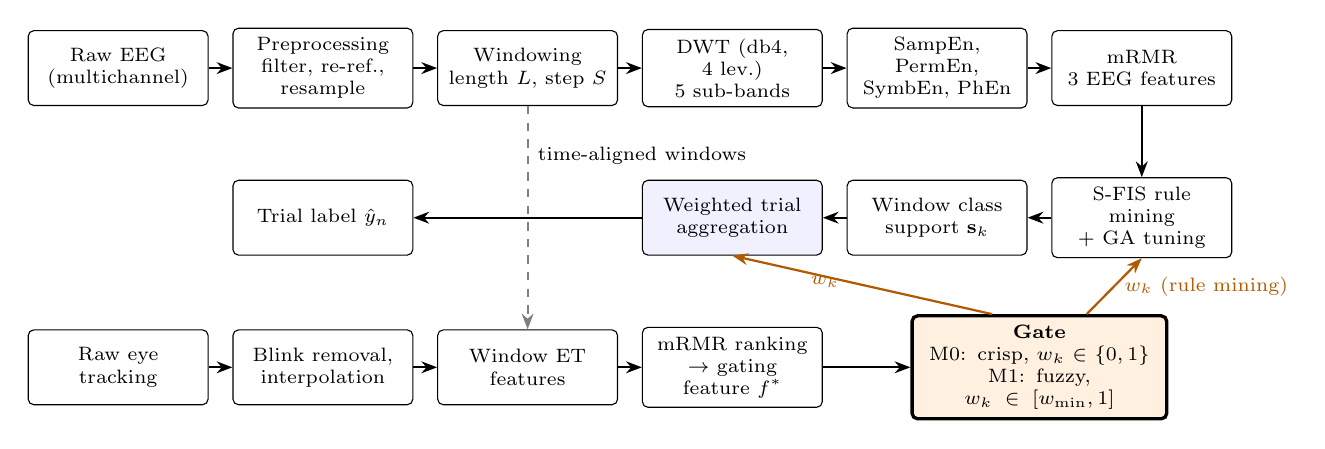
\begin{tikzpicture}[
  font=\scriptsize,
  box/.style={draw, rounded corners=2pt, align=center, minimum height=0.95cm, text width=2.05cm, fill=white},
  gate/.style={draw, very thick, rounded corners=2pt, align=center, minimum height=1.25cm, text width=3.0cm, fill=orange!12},
  arr/.style={-{Stealth[length=2mm]}, thick},
  warr/.style={-{Stealth[length=2mm]}, thick, orange!70!black}]
\def\dx{2.6}
% row 1: EEG feature chain
\node[box] (eeg) at (0,0) {Raw EEG\\(multichannel)};
\node[box] (pre) at (\dx,0) {Preprocessing\\filter, re-ref., resample};
\node[box] (win) at (2*\dx,0) {Windowing\\length $L$, step $S$};
\node[box] (dwt) at (3*\dx,0) {DWT (db4, 4 lev.)\\5 sub-bands};
\node[box] (ent) at (4*\dx,0) {SampEn, PermEn,\\SymbEn, PhEn};
\node[box] (mrmr) at (5*\dx,0) {mRMR\\3 EEG features};
% row 2: classification and aggregation
\node[box] (fis) at (5*\dx,-1.9) {S-FIS rule mining\\+ GA tuning};
\node[box] (sup) at (4*\dx,-1.9) {Window class\\support $\mathbf{s}_k$};
\node[box, fill=blue!6] (agg) at (3*\dx,-1.9) {Weighted trial\\aggregation};
\node[box] (out) at (1*\dx,-1.9) {Trial label $\hat{y}_n$};
% row 3: eye-tracking chain
\node[box] (et) at (0,-3.8) {Raw eye\\tracking};
\node[box] (etp) at (\dx,-3.8) {Blink removal,\\interpolation};
\node[box] (etf) at (2*\dx,-3.8) {Window ET\\features};
\node[box] (etm) at (3*\dx,-3.8) {mRMR ranking\\$\rightarrow$ gating feature $f^\ast$};
\node[gate] (g) at (4.5*\dx,-3.8) {\textbf{Gate}\\M0: crisp, $w_k\in\{0,1\}$\\M1: fuzzy, $w_k\in[w_{\min},1]$};
% arrows
\draw[arr] (eeg)--(pre); \draw[arr] (pre)--(win); \draw[arr] (win)--(dwt); \draw[arr] (dwt)--(ent); \draw[arr] (ent)--(mrmr);
\draw[arr] (mrmr)--(fis); \draw[arr] (fis)--(sup); \draw[arr] (sup)--(agg); \draw[arr] (agg)--(out);
\draw[arr] (et)--(etp); \draw[arr] (etp)--(etf); \draw[arr] (etf)--(etm); \draw[arr] (etm)--(g);
\draw[arr, dashed, gray] (win.south) -- node[pos=0.22, right, text=black]{time-aligned windows} (etf.north);
\draw[warr] ($(g.north)+(0.6,0)$) -- node[right]{$w_k$ (rule mining)} (fis.south);
\draw[warr] ($(g.north)+(-0.6,0)$) -- node[left, pos=0.55]{$w_k$} (agg.south);
\end{tikzpicture}
\caption{Common architecture of the baseline (M0) and the proposed model (M1). All blocks are shared except the gate (shaded), which produces the window weight $w_k$ used in rule mining and in trial-level aggregation.}
\label{fig:arch}
\end{figure}

\begin{table}[t]
\centering\small
\caption{Key notations}\label{tab:notation}
\begin{tabular}{@{}ll@{}}
\toprule
Notation & Description\\
\midrule
$n$, $k$ & Trial (stimulus presentation) index; window index within a trial\\
$K_n$ & Number of windows in trial $n$\\
$\mathbf{x}_{n,k}\in\mathbb{R}^{3}$ & Selected EEG entropy features of window $k$ (S-FIS inputs)\\
$z_{n,k}$, $\tilde z_{n,k}$ & Raw and normalised gating feature $f^\ast$ of window $k$\\
$\tau$ & Hard-gate threshold (M0)\\
$\mu_{L},\mu_{M},\mu_{H}$ & Low/Medium/High membership functions of the gate (M1)\\
$r_{L},r_{M},r_{H}$ & Constant consequents (relevance levels) of the gate rules\\
$w_{n,k}$ & Window weight: $\{0,1\}$ in M0, $[w_{\min},1]$ in M1\\
$\alpha_j(\mathbf{x})$ & Firing strength of classification rule $j$\\
$s_{n,k,c}$ & Support of window $k$ for class $c$\\
$S_{n,c}$ & Aggregated trial support for class $c$\\
$C$ & Number of classes\\
\bottomrule
\end{tabular}
\end{table}

\subsection{Baseline model (M0)}
M0 re-implements the pipeline of \cite{FarhadiSedehi2024a}. Where that description is incomplete, our choice is stated explicitly and marked for confirmation against the team's code.

\paragraph{EEG preprocessing.}
Following \cite{FarhadiSedehi2024a}, EEG is band-pass filtered with a fourth-order Butterworth filter (1--60~Hz), notch-filtered at the power-line frequency, re-referenced to the common average and downsampled to 128~Hz. Filtering is applied with zero phase \pending{confirm zero-phase filtering in code}. For \dataset{}, the corpus provides both raw and preprocessed EEG \cite{Hollenstein2018}; \pending{state whether raw EEG or the provided Automagic/MARA-preprocessed EEG \cite{Pedroni2019,Winkler2011} is used, and whether the baseline filtering is applied on top of it}.

\paragraph{Windowing.}
Each trial is segmented into windows of length $L$ with step $S$. The baseline uses $L=4$~s without stated overlap. \pending{final $L$ and $S$; see Sect.~\ref{sec:data} on trial durations}.

\paragraph{Band decomposition.}
Each window is decomposed by a four-level DWT with the Daubechies-4 mother wavelet \cite{Mallat1989}. At $f_s=128$~Hz the dyadic sub-bands are D1 (32--64~Hz, gamma), D2 (16--32~Hz, beta), D3 (8--16~Hz, alpha), D4 (4--8~Hz, theta) and A4 (0--4~Hz, delta). These dyadic boundaries only approximate the conventional bands quoted in \cite{FarhadiSedehi2024a} (alpha 8--13~Hz, beta 13--25~Hz, gamma 25--60~Hz). Entropies are computed on the single-branch reconstructed sub-band signals, which have the full window length, rather than on the decimated coefficients \pending{confirm in code}. This matters because a level-3 coefficient vector of a 4-s window contains only 64 samples, which is too short for reliable sample and permutation entropy with $m=5$.

\paragraph{Entropy features.}
For each channel and sub-band, four entropies are computed with the parameters of \cite{FarhadiSedehi2024a}. Sample entropy \cite{Richman2000} is
\begin{equation}
\mathrm{SampEn}(m,r,N) = -\ln\frac{A}{B},
\end{equation}
where $B$ and $A$ are the numbers of template pairs of length $m$ and $m+1$ whose Chebyshev distance is below $r$ (self-matches excluded), with $m=5$, delay $2$ and $r=0.15\,\sigma$. Permutation entropy \cite{Bandt2002} is
\begin{equation}
\mathrm{PermEn} = -\sum_{i=1}^{m!} p_i \ln p_i,
\end{equation}
where $p_i$ is the relative frequency of the $i$-th ordinal pattern of order $m=5$ and delay $2$ \pending{state whether normalised by $\ln m!$}. Symbolic dynamics entropy \cite{Zebrowski2000} is the Shannon entropy of symbol words of length $m=5$ and delay $2$ over an alphabet of size $3$. Phase entropy \cite{Rohila2019} is
\begin{equation}
\mathrm{PhEn} = -\sum_{i=1}^{k} p(i)\log p(i),
\end{equation}
where $p(i)$ is the normalised sum of slope angles of the second-order difference plot falling in sector $i$, with $k=5$ sectors. With $N_{ch}$ channels, each window yields $4\times5\times N_{ch}$ features.

\paragraph{Feature selection.}
mRMR \cite{Peng2005} incrementally selects features maximising relevance minus redundancy:
\begin{equation}
f_{t+1} = \arg\max_{f_j\notin\mathcal{S}_t}\Big[I(f_j;y) - \frac{1}{|\mathcal{S}_t|}\sum_{f_i\in\mathcal{S}_t} I(f_j;f_i)\Big],
\end{equation}
where $I(\cdot;\cdot)$ is mutual information, $y$ is the class label and $\mathcal{S}_t$ is the current subset. As in the baseline, three EEG features are retained because the rule base grows exponentially with the number of inputs ($3^3=27$ antecedent combinations). mRMR is run separately per frequency band and \emph{inside each training fold} \pending{confirm per-band vs.\ pooled selection in code}.

\paragraph{Sugeno fuzzy classifier and GA tuning.}
Each selected feature is partitioned into three triangular fuzzy sets (Low, Medium, High) whose split points are obtained by entropy-based discretisation of the training data \cite{FarhadiSedehi2024a}. Candidate rules of the form
\begin{equation}
R_j:\ \text{IF } x_1 \text{ is } A_{j1} \text{ AND } x_2 \text{ is } A_{j2} \text{ AND } x_3 \text{ is } A_{j3} \text{ THEN class} = c_j
\end{equation}
are generated from training windows with a look-up-table procedure \cite{WangMendel1992}. Conflicting rules with identical antecedents are resolved in favour of the rule with the larger accumulated degree. A GA then selects a rule subset, with the initial chromosomes encoding the compatible mined rules and a fitness that combines training accuracy and rule coverage \cite{FarhadiSedehi2024a}. The firing strength of rule $j$ for window input $\mathbf{x}$ is
\begin{equation}
\alpha_j(\mathbf{x}) = \prod_{i=1}^{3}\mu_{A_{ji}}(x_i),
\label{eq:firing}
\end{equation}
and the class support of window $k$ of trial $n$ is
\begin{equation}
s_{n,k,c} = \max_{j:\,c_j=c}\ \alpha_j(\mathbf{x}_{n,k}),\qquad c=1,\dots,C.
\label{eq:support}
\end{equation}
\pending{Confirm the t-norm (product vs.\ minimum), the conflict-resolution score, the GA encoding, population size, crossover and mutation rates, and the exact fitness weighting used in our implementation; the baseline reports only a population derived from the 27 antecedent combinations and termination after 10 generations without fitness improvement.} The baseline describes centroid defuzzification of the Sugeno output; for multi-class decisions we use the class-support formulation of Eq.~\eqref{eq:support}, which yields one score per class and therefore supports aggregation over windows.

\paragraph{Hard eye-tracking gate.}
The baseline extracts eight eye-tracking features per 4-s segment: the mean and standard deviation of fixation duration, fixation frequency, maximum fixation duration, and the mean and standard deviation of pupil diameter in the horizontal and vertical directions \cite{FarhadiSedehi2024a}. The features are ranked with mRMR and the top-ranked feature $f^\ast$ (mean vertical pupil diameter on both of the original datasets) is used as the gate. The original text states that the maximum of this feature is used as a threshold and that EEG at the moments when the feature reaches this maximum is analysed. It does not specify whether the maximum is taken per trial, per subject or over the dataset, nor how many windows follow each marked moment. We therefore formalise the gate generically as
\begin{equation}
w^{\mathrm{M0}}_{n,k} = g^{H}(\tilde z_{n,k}) = \mathbf{1}\big[\tilde z_{n,k}\ \geq\ \tau\big],
\label{eq:hard}
\end{equation}
where $\tilde z_{n,k}$ is the normalised gating feature of window $k$ (Eq.~\eqref{eq:norm}) and $\tau$ is the threshold. \pending{State exactly how $\tau$ is set in our implementation (e.g., per-trial maximum with tolerance, per-subject percentile) and how it is tuned on training folds only.} Windows with $w_{n,k}=0$ are excluded from rule mining and from trial-level aggregation. If a trial has no window above $\tau$, the window with the largest $\tilde z_{n,k}$ is retained so that every trial receives a prediction.

\subsection{Proposed fuzzy-gating model (M1)}
M1 keeps every component of M0 and replaces Eq.~\eqref{eq:hard} with a fuzzy gate. To isolate the effect of the gating function, the gate input is the same feature $f^\ast$ selected by mRMR in M0.

\paragraph{Eye-tracking preprocessing and normalisation.}
Blink and missing pupil samples are removed and short gaps are linearly interpolated \cite{Kret2019}. Windows with more than \pending{maximum fraction of invalid samples} invalid samples are flagged. Because absolute pupil size varies strongly between individuals and recording sessions \cite{Mathot2018}, the window-level feature $z_{n,k}$ is normalised per subject with robust percentile scaling:
\begin{equation}
\tilde z_{n,k} = \operatorname{clip}_{[0,1]}\left(\frac{z_{n,k}-P_{5}^{(s)}}{P_{95}^{(s)}-P_{5}^{(s)}}\right),
\label{eq:norm}
\end{equation}
where $P_{5}^{(s)}$ and $P_{95}^{(s)}$ are the 5th and 95th percentiles of the feature over all windows of subject $s$. The percentiles use no labels. For a held-out test subject they are computed from that subject's unlabelled eye-tracking data, a label-free, subject-wise calibration step that is applied identically in M0 and M1 \pending{confirm normalisation scheme in code}.

\paragraph{Fuzzification.}
The normalised feature is described by three fuzzy sets with trapezoidal shoulders and a triangular centre (Fig.~\ref{fig:mf}a):
\begin{align}
\mu_{L}(\tilde z) &= \max\!\Big(0,\min\!\Big(1,\frac{b_1-\tilde z}{b_1-a_1}\Big)\Big),\\
\mu_{M}(\tilde z) &= \max\!\Big(0,\min\!\Big(\frac{\tilde z-a_1}{c-a_1},\frac{b_2-\tilde z}{b_2-c}\Big)\Big),\\
\mu_{H}(\tilde z) &= \max\!\Big(0,\min\!\Big(1,\frac{\tilde z-a_2}{b_2-a_2}\Big)\Big),
\end{align}
with $0\le a_1<c<b_2\le1$, $b_1=c$ and $a_2=c$, so that the three sets form a Ruspini partition ($\mu_L+\mu_M+\mu_H=1$). The illustrative values in Fig.~\ref{fig:mf} are $a_1=0.2$, $c=0.5$ and $b_2=0.8$. \pending{Final MF shape and parameters as implemented, and whether they are fixed a priori, set from training-fold percentiles, or tuned on an inner validation split.}

\paragraph{Gate rule base and weight computation.}
A zero-order Sugeno rule base maps the memberships to a relevance level:
\begin{align*}
&R^{g}_1:\ \text{IF } \tilde z_{n,k} \text{ is Low THEN relevance} = r_L,\\
&R^{g}_2:\ \text{IF } \tilde z_{n,k} \text{ is Medium THEN relevance} = r_M,\\
&R^{g}_3:\ \text{IF } \tilde z_{n,k} \text{ is High THEN relevance} = r_H,
\end{align*}
with $0<r_L<r_M<r_H=1$. The window weight is the weighted-average defuzzification
\begin{equation}
w^{\mathrm{M1}}_{n,k} = \frac{\mu_L(\tilde z_{n,k})\,r_L + \mu_M(\tilde z_{n,k})\,r_M + \mu_H(\tilde z_{n,k})\,r_H}{\mu_L(\tilde z_{n,k})+\mu_M(\tilde z_{n,k})+\mu_H(\tilde z_{n,k})}\ \in [r_L,1],
\label{eq:fuzzy}
\end{equation}
so $w_{\min}=r_L>0$ guarantees that no window is entirely discarded. The illustrative values in Fig.~\ref{fig:mf}b are $r_L=0.1$, $r_M=0.5$ and $r_H=1$. \pending{Final consequents as implemented.} Windows flagged for poor eye-tracking quality receive the neutral weight $r_M$, expressing that their relevance is unknown \pending{confirm handling of low-quality windows}.

Two properties follow from Eq.~\eqref{eq:fuzzy}. First, if the Medium set shrinks to zero width at $\tau$ and $r_L\to0$, the gate reduces to the crisp step of Eq.~\eqref{eq:hard}, so M0 is a limiting case of M1. Second, with one input and a Ruspini partition, Eq.~\eqref{eq:fuzzy} is a monotone piecewise-linear function of $\tilde z$. The single-input fuzzy gate is therefore equivalent to a particular soft threshold with linguistically interpretable parameters. Its value over other soft thresholds is not guaranteed and is examined in the ablation study (Sect.~\ref{sec:ablation}). \pending{If the implementation uses two gate inputs (e.g., pupil feature and mean fixation duration) with a $3\times3$ rule table, replace this paragraph with the two-input rule table and its consequents.}

\begin{figure}[t]
\centering
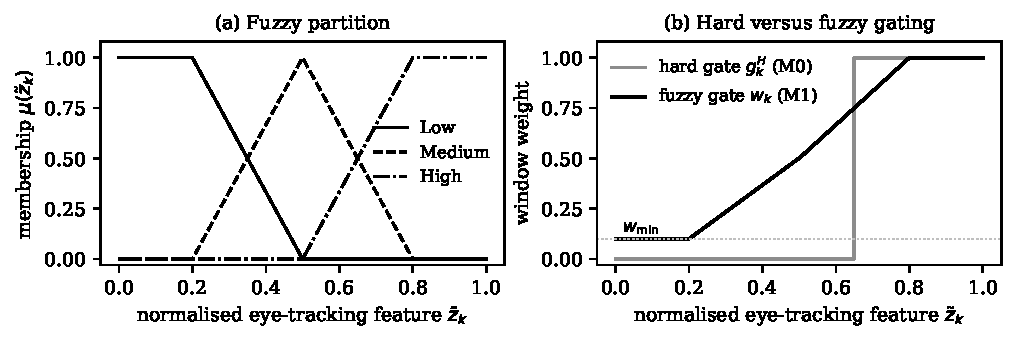
\includegraphics[width=0.95\linewidth]{figures/fuzzy_gate_mf.pdf}
\caption{(a) Fuzzy partition of the normalised gating feature into Low, Medium and High sets. (b) Resulting window weight of the fuzzy gate (Eq.~\ref{eq:fuzzy}) compared with the hard gate (Eq.~\ref{eq:hard}). The parameters ($a_1=0.2$, $c=0.5$, $b_2=0.8$, $r=(0.1,0.5,1)$, $\tau=0.65$) are illustrative design values, not fitted to data.}
\label{fig:mf}
\end{figure}

\paragraph{Integration of weights into rule mining.}
In M0, windows with $w=0$ are removed from the training set. In M1 every training window contributes in proportion to its weight. In the look-up-table rule generation, the degree of a candidate rule generated by window $k$ becomes $w_{n,k}\,\alpha_j(\mathbf{x}_{n,k})$, and the GA fitness uses weighted accuracy and weighted coverage:
\begin{equation}
\mathrm{Acc}_w = \frac{\sum_{n,k} w_{n,k}\,\mathbf{1}[\hat y_{n,k}=y_n]}{\sum_{n,k} w_{n,k}},\qquad
\mathrm{Cov}_w = \frac{\sum_{n,k} w_{n,k}\,\mathbf{1}[\exists j:\alpha_j(\mathbf{x}_{n,k})>0]}{\sum_{n,k} w_{n,k}}.
\label{eq:wfit}
\end{equation}
With $w\in\{0,1\}$, Eq.~\eqref{eq:wfit} reduces to the unweighted fitness computed on the retained windows of M0. \pending{Confirm whether weights are used in training, at inference only, or both; if only at inference, delete this paragraph and add the training-weight variant to the ablation list.}

\paragraph{Weighted trial-level aggregation.}
The trial prediction is obtained by weighted aggregation of window class supports:
\begin{equation}
S_{n,c} = \frac{\sum_{k=1}^{K_n} w_{n,k}\,s_{n,k,c}}{\sum_{k=1}^{K_n} w_{n,k}},\qquad
\hat y_n = \arg\max_{c} S_{n,c}.
\label{eq:agg}
\end{equation}
Equation~\eqref{eq:agg} is a weighted sum rule in the sense of \cite{Kittler1998}. M0 uses the same equation with binary weights, so both models produce exactly one prediction per trial and are evaluated on the same set of trials. Algorithm~\ref{alg:m1} summarises the procedure for one cross-validation fold.

\begin{algorithm}[t]
\caption{Fuzzy-gated S-FIS-GA emotion recognition (one CV fold)}\label{alg:m1}
\small
\begin{algorithmic}[1]
\Require Training trials $\mathcal{T}$, test trials $\mathcal{V}$ (disjoint subjects/stimuli), gate parameters $\theta_g$
\Ensure Trial predictions $\{\hat y_n\}_{n\in\mathcal{V}}$
\State Preprocess EEG and ET; segment every trial into windows $k=1..K_n$
\For{each window} compute ET features and DWT-band entropy features \EndFor
\State Rank ET features by mRMR on $\mathcal{T}$; select gating feature $f^\ast$
\State Normalise $f^\ast$ per subject (Eq.~\ref{eq:norm}) $\rightarrow \tilde z_{n,k}$
\State $w_{n,k}\gets$ Eq.~\eqref{eq:hard} (M0) \textbf{or} Eq.~\eqref{eq:fuzzy} (M1)
\State Select 3 EEG features per band by mRMR on $\mathcal{T}$ (weighted windows)
\State Fit discretisation split points and triangular MFs on $\mathcal{T}$
\State Mine look-up-table rules with degrees $w_{n,k}\alpha_j$; resolve conflicts
\State Optimise rule subset with GA using fitness from Eq.~\eqref{eq:wfit}
\For{each test trial $n\in\mathcal{V}$}
  \State compute $s_{n,k,c}$ (Eq.~\ref{eq:support}) for all windows; aggregate with Eq.~\eqref{eq:agg}; $\hat y_n\gets\arg\max_c S_{n,c}$
\EndFor
\end{algorithmic}
\end{algorithm}

\subsection{Unchanged and modified components}
Table~\ref{tab:m0m1} lists the components of the two models. The only modified component is the gate function. The fallback rule of M0 (keep the best window when none passes) and the aggregation of Eq.~\eqref{eq:agg} are additions needed so that both models produce trial-level predictions on the same trials; they are applied identically to both.

\begin{table}[t]
\centering\small
\caption{Components of the baseline (M0) and proposed (M1) models}\label{tab:m0m1}
\begin{tabular}{@{}lll@{}}
\toprule
Component & M0 (baseline) & M1 (proposed)\\
\midrule
EEG preprocessing, windowing & as \cite{FarhadiSedehi2024a} & unchanged\\
DWT (db4, 4 levels), 4 entropies & as \cite{FarhadiSedehi2024a} & unchanged\\
EEG mRMR (3 features) & as \cite{FarhadiSedehi2024a} & unchanged\\
S-FIS (3 triangular MFs, look-up rules) + GA & as \cite{FarhadiSedehi2024a} & unchanged\\
ET features and mRMR ranking & as \cite{FarhadiSedehi2024a}$^\ddagger$ & unchanged\\
\textbf{Gate} & crisp, $w\in\{0,1\}$ (Eq.~\ref{eq:hard}) & \textbf{fuzzy, $w\in[r_L,1]$ (Eq.~\ref{eq:fuzzy})}\\
Use of $w$ in training & window removal & weighted rule degree / fitness\\
Trial aggregation & Eq.~\eqref{eq:agg}, binary $w$ & Eq.~\eqref{eq:agg}, continuous $w$\\
\bottomrule
\multicolumn{3}{@{}l}{\scriptsize $^\ddagger$ adapted to the eye-tracking variables available in the dataset (Sect.~\ref{sec:data}).}
\end{tabular}
\end{table}

% =====================================================================
\section{Dataset description}
\label{sec:data}

\pending{The team must confirm the dataset. The name ``Zuko'' is taken to refer to the Zurich Cognitive Language Processing Corpus (ZuCo). No public EEG and eye-tracking dataset named ``Zuko'' was found. If the intended dataset is SEED-IV, replace this section; see the accompanying research notes.}

ZuCo~1.0 \cite{Hollenstein2018} is a freely available corpus of simultaneous EEG and eye-tracking recordings acquired during natural sentence reading. It is distributed under a CC~BY~4.0 licence through the Open Science Framework (\url{https://osf.io/q3zws}). Twelve healthy, right-handed native English speakers (5 female, aged 22--54 years) read sentences presented one at a time on a screen. EEG was recorded with a 128-channel EGI Geodesic HydroCel system at 500~Hz with a 0.1--100~Hz online band-pass and Cz reference. After exclusion of peripheral and ocular channels, 105 scalp channels are used, and 9 EOG channels are available. The corpus provides raw data and data preprocessed with Automagic \cite{Pedroni2019}, which includes MARA-based independent-component artefact rejection \cite{Winkler2011}, high-pass and notch filtering and bad-channel interpolation. Eye movements were recorded with an EyeLink~1000~Plus at 500~Hz. The corpus provides raw samples, fixation-level word measures (first fixation duration, single fixation duration, gaze duration, go-past time, total reading time and number of fixations) and pupil size at word and sentence level \cite{Hollenstein2018}.

The corpus contains three reading tasks. Only the sentiment-reading (SR) task carries affect-related labels. It comprises 400 movie-review sentences from the Stanford Sentiment Treebank \cite{Socher2013} labelled positive (140), negative (137) or neutral (123). These labels describe the \emph{sentiment of the text}, inherited from the treebank annotation; they are not self-reports of the reader's emotional state. Participants rated the quality of the reviewed movie for 47 sentences only, with 79.53\% agreement with the treebank labels \cite{Hollenstein2018}. ZuCo~2.0 \cite{Hollenstein2020} adds 18 participants but contains no sentiment task. Table~\ref{tab:dataset} summarises the characteristics relevant to this study.

\begin{table}[t]
\centering\small
\caption{Characteristics of the ZuCo~1.0 sentiment-reading task as used in this study}\label{tab:dataset}
\begin{tabular}{@{}ll@{}}
\toprule
Property & Value\\
\midrule
Participants & 12 (5 F / 7 M), 22--54 years \cite{Hollenstein2018}; usable: \pending{number after QC}\\
EEG & EGI HydroCel 128-ch, 500 Hz, 105 scalp channels used\\
Eye tracker & EyeLink 1000 Plus, 500 Hz, gaze and pupil size\\
Stimuli & 400 sentences (Stanford Sentiment Treebank \cite{Socher2013})\\
Classes & positive 140 / negative 137 / neutral 123 (stimulus sentiment)\\
Trial definition & one sentence reading period \pending{confirm}\\
Trial duration & \pending{mean $\pm$ SD reading time per sentence}\\
Windows per trial & \pending{distribution of $K_n$ for the chosen $L$, $S$}\\
Format, licence & MATLAB files on OSF; CC BY 4.0\\
\bottomrule
\end{tabular}
\end{table}

\paragraph{Consequences for the experimental design.}
Four differences from the baseline datasets affect the study and are stated here rather than hidden. (i) The classification target becomes three-class \emph{stimulus sentiment} (positive, neutral, negative) instead of the four induced emotions (happiness, sadness, fear, neutral); results are therefore not comparable with the 94.42\% reported on SEED-IV \cite{FarhadiSedehi2024a}. (ii) Sentences are read in a few seconds, so 4-s windows may yield only one or two windows per trial, which limits the scope of any window gate; the window length must be chosen from the measured reading-time distribution \pending{decision on $L$}. (iii) EyeLink provides a single pupil-size value rather than separate horizontal and vertical diameters, so the eight baseline eye-tracking features reduce to six (mean and standard deviation of fixation duration, fixation frequency, maximum fixation duration, and mean and standard deviation of pupil size) \pending{confirm feature list}. (iv) The baseline channels T7, T8 and Fp2 have no exact counterparts in the HydroCel 128 montage, so EEG feature selection is rerun on the ZuCo channels. During reading, pupil size is further modulated by cognitive load and by gaze position on the screen, which strengthens the case for treating it as an uncertain indicator.

% =====================================================================
\section{Experimental setup}
\label{sec:setup}

\subsection{Configurations}
Two primary configurations are compared: M0 (hard gate, Eq.~\ref{eq:hard}) and M1 (fuzzy gate, Eq.~\ref{eq:fuzzy}). Both share all components listed in Table~\ref{tab:m0m1} and all hyperparameters in Table~\ref{tab:hyper}. A no-gate reference (all $w_{n,k}=1$) is also reported to show whether eye-tracking gating of any kind is beneficial.

\begin{table}[t]
\centering\small
\caption{Hyperparameters (baseline values from \cite{FarhadiSedehi2024a} unless stated)}\label{tab:hyper}
\begin{tabularx}{\linewidth}{@{}llX@{}}
\toprule
Stage & Parameter & Value\\
\midrule
Preprocessing & Band-pass / notch / resampling & 1--60 Hz Butterworth (4th order) / \pending{50 Hz} / 128 Hz\\
Windowing & Length $L$ / step $S$ & \pending{} / \pending{}\\
DWT & Wavelet, levels & db4, 4\\
SampEn & $m$, delay, $r$ & 5, 2, $0.15\sigma$\\
PermEn & $m$, delay & 5, 2\\
SymbEn & $m$, delay, alphabet & 5, 2, 3\\
PhEn & sectors $k$ & 5\\
mRMR & EEG features retained & 3 per band\\
S-FIS & MFs per input, shape & 3, triangular (entropy-based split points)\\
GA & population / crossover / mutation & \pending{} / \pending{} / \pending{}\\
GA & termination & no fitness gain in 10 generations\\
Hard gate (M0) & threshold rule $\tau$ & \pending{}\\
Fuzzy gate (M1) & $a_1, c, b_2$ / $r_L, r_M, r_H$ & \pending{} / \pending{}\\
\bottomrule
\end{tabularx}
\end{table}

\subsection{Validation protocol and leakage control}
Windows from the same trial are strongly correlated, and in ZuCo every participant reads the same 400 sentences. A random split of windows would therefore place near-duplicate information in the training and test sets \cite{Li2021,Khan2025}. The baseline evaluated 5-fold CV over pooled segments \cite{FarhadiSedehi2024a}, which does not exclude this. We use the following protocols.
\begin{itemize}
  \item \textbf{P1 (primary): subject- and sentence-disjoint CV.} Sentences are partitioned into 5 stratified folds. For each held-out subject and each sentence fold, models are trained on the remaining subjects' windows from the remaining sentence folds and tested on the held-out subject's windows from the held-out sentence fold ($12\times5$ train--test runs). Neither the test subject nor the test sentences are seen during training.
  \item \textbf{P2: within-subject, sentence-grouped 5-fold CV}, reported per subject, to estimate subject-dependent performance without trial leakage.
  \item \textbf{P3 (replication only): window-level random 5-fold CV} as in \cite{FarhadiSedehi2024a}, reported solely to quantify the optimism of the original protocol. P3 is not used to compare M0 and M1.
\end{itemize}
In every protocol, all data-dependent steps are fitted on the training portion only: eye-tracking and EEG mRMR selection, discretisation split points, membership functions, the hard threshold $\tau$, any tuned fuzzy-gate parameters (using an inner split of the training subjects) and the GA. The only step that touches test data without labels is the per-subject percentile normalisation of Eq.~\eqref{eq:norm}, applied identically to M0 and M1. M0 and M1 use identical folds and random seeds. \pending{GA random seeds and number of repetitions.}

\subsection{Evaluation metrics}
Performance is measured at trial level (one prediction per sentence) and, secondarily, at window level. For $C$ classes with per-class true positives $tp_c$, false positives $fp_c$ and false negatives $fn_c$:
\begin{gather}
\mathrm{Acc} = \frac{\sum_c tp_c}{N},\quad
P_c = \frac{tp_c}{tp_c+fp_c},\quad
R_c = \frac{tp_c}{tp_c+fn_c},\quad
F1_c = \frac{2P_cR_c}{P_c+R_c},\\
\text{macro-}F1 = \frac{1}{C}\sum_{c}F1_c,\qquad
\text{BalAcc} = \frac{1}{C}\sum_c R_c .
\end{gather}
Macro-averaged precision, recall and F1 and balanced accuracy are reported because the classes are not perfectly balanced. The majority-class rate (35.0\% for positive) and a label-permutation test give the empirical chance level. Confusion matrices are accumulated over all test folds. Computational cost is reported as wall-clock time for feature extraction, rule mining and GA tuning and for inference per trial, together with the gate retention ratio $\rho=\frac{1}{\sum_n K_n}\sum_{n,k}\mathbf{1}[w_{n,k}>0]$ for M0 and the effective number of windows $\sum_{n,k}w_{n,k}$ for M1.

\subsection{Statistical analysis}
M0 and M1 are compared with the Wilcoxon signed-rank test on per-subject macro-F1 under P1 (12 paired observations), as recommended for comparing two classifiers over multiple data partitions \cite{Demsar2006}, and with McNemar's test on pooled paired trial predictions \cite{McNemar1947}. Effect sizes (median paired difference with a bootstrap 95\% confidence interval) are reported alongside $p$-values. With 12 subjects the tests have limited power, so a non-significant difference will be reported as inconclusive rather than as evidence of equivalence.

\subsection{Ablation study}
\label{sec:ablation}
To attribute any difference to the fuzzy formulation rather than to softness alone, the following variants are planned \pending{confirm which are run}: (A1) no gate; (A2) M0; (A3) M1; (A4) linear soft gate $w=\max(r_L,\tilde z)$; (A5) M1 weights used at inference only; (A6) M1 weights used in training only; (A7) sensitivity of M1 to $r_L\in\{0,0.1,0.3\}$ and to the width of the Medium set.

\subsection{Implementation environment}
\pending{Programming language and versions; libraries for DWT, entropy, mRMR, fuzzy inference and GA; CPU/GPU, RAM and operating system; code repository link.}

% =====================================================================
\section{Results and discussion}
\label{sec:results}

\revise{This section contains placeholders only. No values are estimated. Populate from the experiment logs.}

\subsection{Eye-tracking feature ranking}
\pending{mRMR ranking of eye-tracking features on \dataset{} (cf.\ Fig.~7 of \cite{FarhadiSedehi2024a}); state which feature is selected as $f^\ast$ and whether the selection is stable across folds.} \pending{Figure: distribution of $\tilde z_{n,k}$ per class and gate weights for M0 and M1.}

\subsection{Overall comparison}
Table~\ref{tab:main} will report the primary comparison under protocol P1.

\begin{table}[t]
\centering\small
\caption{Trial-level performance under protocol P1 (mean $\pm$ SD over subjects). Values are placeholders.}\label{tab:main}
\begin{tabular}{@{}lccc@{}}
\toprule
Metric & No gate (A1) & Baseline M0 (hard gate) & Proposed M1 (fuzzy gate)\\
\midrule
Accuracy (\%) & \PND & \PND & \PND\\
Balanced accuracy (\%) & \PND & \PND & \PND\\
Macro precision (\%) & \PND & \PND & \PND\\
Macro recall (\%) & \PND & \PND & \PND\\
Macro F1 (\%) & \PND & \PND & \PND\\
Training time (s) & \PND & \PND & \PND\\
Inference time per trial (ms) & \PND & \PND & \PND\\
Retained / effective windows (\%) & 100 & \PND & \PND\\
\bottomrule
\end{tabular}
\end{table}

\pending{Baseline accuracy}; \pending{Proposed model accuracy}; \pending{Precision, recall and F1-score}. \revise{Describe the difference between M0 and M1 with its confidence interval; do not describe it as an improvement unless the paired test and effect size support it.}

\subsection{Frequency-band analysis}
\begin{table}[t]
\centering\small
\caption{Macro-F1 (\%) per DWT sub-band under P1. Values are placeholders.}\label{tab:bands}
\begin{tabular}{@{}lccccc@{}}
\toprule
Model & Delta (A4) & Theta (D4) & Alpha (D3) & Beta (D2) & Gamma (D1)\\
\midrule
M0 & \PND & \PND & \PND & \PND & \PND\\
M1 & \PND & \PND & \PND & \PND & \PND\\
\bottomrule
\end{tabular}
\end{table}
\revise{Compare the band ranking with the alpha/beta/gamma dominance reported in \cite{FarhadiSedehi2024a}; state whether the selected channels are plausible for reading.}

\subsection{Class-wise performance and confusion matrices}
\begin{table}[t]
\centering\small
\caption{Class-wise precision / recall / F1 (\%) under P1. Values are placeholders.}\label{tab:class}
\begin{tabular}{@{}lcccccc@{}}
\toprule
 & \multicolumn{3}{c}{M0} & \multicolumn{3}{c}{M1}\\
\cmidrule(lr){2-4}\cmidrule(lr){5-7}
Class & P & R & F1 & P & R & F1\\
\midrule
Positive & \PND & \PND & \PND & \PND & \PND & \PND\\
Neutral  & \PND & \PND & \PND & \PND & \PND & \PND\\
Negative & \PND & \PND & \PND & \PND & \PND & \PND\\
\bottomrule
\end{tabular}
\end{table}
\pending{Confusion matrix} for M0 and M1 (Fig.~\ref{fig:cm}). \revise{Discuss which classes are confused, e.g., whether neutral is absorbed by positive or negative, and whether the fuzzy gate changes the error pattern.}

\begin{figure}[t]
\centering
\fbox{\parbox[c][3.2cm][c]{0.44\linewidth}{\centering\PND\\ Confusion matrix, M0 (P1)}}\hfill
\fbox{\parbox[c][3.2cm][c]{0.44\linewidth}{\centering\PND\\ Confusion matrix, M1 (P1)}}
\caption{Trial-level confusion matrices accumulated over all P1 test folds. Placeholder.}
\label{fig:cm}
\end{figure}

\subsection{Statistical significance and per-subject results}
\pending{Statistical significance, if evaluated}: Wilcoxon signed-rank statistic, $p$-value and median paired difference with 95\% CI; McNemar $\chi^2$ and $p$. \pending{Figure: paired per-subject macro-F1 of M0 vs.\ M1.}

\subsection{Effect of the validation protocol}
\begin{table}[t]
\centering\small
\caption{Accuracy (\%) of M0 and M1 under the three protocols. Values are placeholders.}\label{tab:protocol}
\begin{tabular}{@{}lccc@{}}
\toprule
Model & P1 (subject+sentence disjoint) & P2 (within-subject) & P3 (window-random, leaky)\\
\midrule
M0 & \PND & \PND & \PND\\
M1 & \PND & \PND & \PND\\
\bottomrule
\end{tabular}
\end{table}
\revise{Quantify the gap between P3 and P1 and discuss its implication for previously reported accuracies.}

\subsection{Ablation and sensitivity}
\pending{Comparative analysis}: results of A1--A7. \revise{State whether M1 differs from the linear soft gate (A4). If not, report that the benefit, if any, comes from soft weighting rather than from the fuzzy formulation itself.}

\subsection{Computational cost}
\pending{Computational cost}. \revise{The baseline argues that gating reduces computation by discarding windows \cite{FarhadiSedehi2024a}; M1 processes every window, so report the cost--accuracy trade-off explicitly.}

\subsection{Discussion}
\revise{Interpret the findings against the hypothesis. Address: (1) whether graded gating helped, matched or degraded performance and for which classes; (2) whether the gate weights relate to labels at all on reading data; (3) interpretability of the gate rules; (4) unexpected findings. Every claim must be traceable to Tables~\ref{tab:main}--\ref{tab:protocol}.}

% =====================================================================
\section{Limitations}
\label{sec:limits}
\paragraph{Known limitations.}
(i) \dataset{} labels describe the sentiment of the text read, not the participant's induced emotion, and the four emotional categories of the baseline are not available; conclusions about emotion recognition in the sense of \cite{FarhadiSedehi2024a} can therefore not be drawn from this dataset alone. (ii) The sample of 12 participants limits statistical power and generalisation. (iii) The baseline description leaves the threshold rule, GA settings and several implementation details unspecified, so M0 is a faithful re-implementation of the published description rather than a reproduction of the original code. (iv) Pupil size is affected by luminance, gaze position and cognitive load \cite{Mathot2018,Raiturkar2016}, none of which is explicitly corrected in either model. (v) The S-FIS restricts the classifier to three EEG inputs, as acknowledged in \cite{FarhadiSedehi2024a}. (vi) A single-input fuzzy gate is mathematically a piecewise-linear soft threshold, so its added value over simpler soft weighting must be shown empirically.

\paragraph{Potential limitations requiring experimental investigation.}
(a) Short sentence durations may yield too few windows per trial for gating to matter. (b) Entropy estimates on short windows may be unstable. (c) The membership parameters may need tuning, which increases the risk of overfitting with few subjects. (d) The gating feature selected by mRMR may vary across folds. (e) Retaining all windows in M1 increases computational cost relative to M0. \revise{Update according to observed results.}

% =====================================================================
\section{Conclusion and future work}
\label{sec:conclusion}
This paper investigated whether the hard eye-tracking threshold used to select EEG segments in a fuzzy rule-mining emotion-recognition pipeline can be replaced by a fuzzy gate that assigns each EEG window a continuous relevance weight. The proposed gate fuzzifies the normalised eye-tracking feature into Low, Medium and High sets, maps the memberships to a weight with a zero-order Sugeno rule base, and applies the weight in rule mining and in trial-level aggregation. All other components of the baseline are left unchanged, and the hard gate is a limiting case of the fuzzy gate. Both models are evaluated on the publicly available \dataset{} corpus under subject- and stimulus-disjoint cross-validation that prevents window-level leakage. \revise{Summarise the measured effect of fuzzy gating, its statistical support, and its cost.}

Future work will \revise{adjust to results}: evaluate the gate on emotion-induction corpora with self-reported labels such as SEED-IV \cite{Zheng2019} and MAHNOB-HCI \cite{Soleymani2012db}; correct the pupil signal for luminance before gating \cite{Raiturkar2016}; extend the gate to several eye-tracking inputs; and learn the membership parameters with neuro-fuzzy methods \cite{Jang1993} under nested cross-validation.

% =====================================================================
\section*{Declarations}
\noindent\textbf{Funding} \pending{}\\
\textbf{Conflict of interest} \pending{}\\
\textbf{Data availability} ZuCo~1.0 is publicly available at \url{https://osf.io/q3zws} under CC~BY~4.0 \cite{Hollenstein2018}.\\
\textbf{Code availability} \pending{repository link}\\
\textbf{Author contributions} \pending{}

% =====================================================================
\small
\begin{thebibliography}{99}

\bibitem{Alarcao2019} Alarc\~ao SM, Fonseca MJ (2019) Emotions recognition using EEG signals: a survey. IEEE Trans Affect Comput 10(3):374--393. \url{https://doi.org/10.1109/TAFFC.2017.2714671}

\bibitem{Arevalo2020} Arevalo J, Solorio T, Montes-y-G\'omez M, Gonz\'alez FA (2020) Gated multimodal networks. Neural Comput Appl 32(14):10209--10228. \url{https://doi.org/10.1007/s00521-019-04559-1}

\bibitem{Bandt2002} Bandt C, Pompe B (2002) Permutation entropy: a natural complexity measure for time series. Phys Rev Lett 88(17):174102. \url{https://doi.org/10.1103/PhysRevLett.88.174102}

\bibitem{Bradley2008} Bradley MM, Miccoli L, Escrig MA, Lang PJ (2008) The pupil as a measure of emotional arousal and autonomic activation. Psychophysiology 45(4):602--607. \url{https://doi.org/10.1111/j.1469-8986.2008.00654.x}

\bibitem{ChoKim1995} Cho SB, Kim JH (1995) Combining multiple neural networks by fuzzy integral for robust classification. IEEE Trans Syst Man Cybern 25(2):380--384. \url{https://doi.org/10.1109/21.364825}

\bibitem{Demsar2006} Dem\v{s}ar J (2006) Statistical comparisons of classifiers over multiple data sets. J Mach Learn Res 7:1--30

\bibitem{Duan2013} Duan RN, Zhu JY, Lu BL (2013) Differential entropy feature for EEG-based emotion classification. In: 6th Int IEEE/EMBS Conf Neural Engineering (NER), pp 81--84. \url{https://doi.org/10.1109/NER.2013.6695876}

\bibitem{FarhadiSedehi2024a} Farhadi Sedehi J, Jafarnia Dabanloo N, Maghooli K, Sheikhani A (2024) Recognition of emotional categories using mined fuzzy rules from electroencephalogram signals with gated eye track data approach. IEEE Access 12:118122--118140. \url{https://doi.org/10.1109/ACCESS.2024.3430934}

\bibitem{FarhadiSedehi2024b} Farhadi Sedehi J, Jafarnia Dabanloo N, Maghooli K, Sheikhani A (2024) Multimodal insights into Granger causality connectivity: integrating physiological signals and gated eye-tracking data for emotion recognition using convolutional neural network. Heliyon 10(16):e36411. \url{https://doi.org/10.1016/j.heliyon.2024.e36411}

\bibitem{Fu2023} Fu B, Gu C, Fu M, Xia Y, Liu Y (2023) A novel feature fusion network for multimodal emotion recognition from EEG and eye movement signals. Front Neurosci 17:1234162. \url{https://doi.org/10.3389/fnins.2023.1234162}

\bibitem{Hollenstein2018} Hollenstein N, Rotsztejn J, Troendle M, Pedroni A, Zhang C, Langer N (2018) ZuCo, a simultaneous EEG and eye-tracking resource for natural sentence reading. Sci Data 5:180291. \url{https://doi.org/10.1038/sdata.2018.291}

\bibitem{Hollenstein2020} Hollenstein N, Troendle M, Zhang C, Langer N (2020) ZuCo 2.0: a dataset of physiological recordings during natural reading and annotation. In: Proc 12th Language Resources and Evaluation Conf (LREC), pp 138--146

\bibitem{Holmqvist2012} Holmqvist K, Nystr\"om M, Mulvey F (2012) Eye tracker data quality: what it is and how to measure it. In: Proc Symp Eye Tracking Research and Applications (ETRA), pp 45--52. \url{https://doi.org/10.1145/2168556.2168563}

\bibitem{Jacobs1991} Jacobs RA, Jordan MI, Nowlan SJ, Hinton GE (1991) Adaptive mixtures of local experts. Neural Comput 3(1):79--87. \url{https://doi.org/10.1162/neco.1991.3.1.79}

\bibitem{Jang1993} Jang JSR (1993) ANFIS: adaptive-network-based fuzzy inference system. IEEE Trans Syst Man Cybern 23(3):665--685. \url{https://doi.org/10.1109/21.256541}

\bibitem{Jenke2014} Jenke R, Peer A, Buss M (2014) Feature extraction and selection for emotion recognition from EEG. IEEE Trans Affect Comput 5(3):327--339. \url{https://doi.org/10.1109/TAFFC.2014.2339834}

\bibitem{Kaya2024} Kaya \"U, Akay D, \c{S}eng\"ul Ayan S (2024) EEG-based emotion recognition in neuromarketing using fuzzy linguistic summarization. IEEE Trans Fuzzy Syst 32(8):4248--4259. \url{https://doi.org/10.1109/TFUZZ.2024.3392495}

\bibitem{Khan2025} Khan NN, Sweet T, Harvey CA, Knapp C, Krusienski DJ, Thompson DE (2025) The role of review process failures in affective state estimation: an empirical investigation of DEAP dataset. arXiv:2508.02417 (preprint)

\bibitem{Kittler1998} Kittler J, Hatef M, Duin RPW, Matas J (1998) On combining classifiers. IEEE Trans Pattern Anal Mach Intell 20(3):226--239. \url{https://doi.org/10.1109/34.667881}

\bibitem{Koelstra2012} Koelstra S, M\"uhl C, Soleymani M, Lee JS, Yazdani A, Ebrahimi T, Pun T, Nijholt A, Patras I (2012) DEAP: a database for emotion analysis using physiological signals. IEEE Trans Affect Comput 3(1):18--31. \url{https://doi.org/10.1109/T-AFFC.2011.15}

\bibitem{Kret2019} Kret ME, Sjak-Shie EE (2019) Preprocessing pupil size data: guidelines and code. Behav Res Methods 51(3):1336--1342. \url{https://doi.org/10.3758/s13428-018-1075-y}

\bibitem{Kukhilava2025} Kukhilava N, Tsmindashvili T, Kalandadze R, et al (2025) Evaluation in EEG emotion recognition: state-of-the-art review and unified framework. arXiv:2505.18175 (preprint)

\bibitem{Li2021} Li R, Johansen JS, Ahmed H, Ilyevsky TV, Wilbur RB, Bharadwaj HM, Siskind JM (2021) The perils and pitfalls of block design for EEG classification experiments. IEEE Trans Pattern Anal Mach Intell 43(1):316--333. \url{https://doi.org/10.1109/TPAMI.2020.2973153}

\bibitem{Lim2020} Lim JZ, Mountstephens J, Teo J (2020) Emotion recognition using eye-tracking: taxonomy, review and current challenges. Sensors 20(8):2384. \url{https://doi.org/10.3390/s20082384}

\bibitem{LinWang2002} Lin CF, Wang SD (2002) Fuzzy support vector machines. IEEE Trans Neural Netw 13(2):464--471. \url{https://doi.org/10.1109/72.991432}

\bibitem{Liu2022} Liu W, Qiu JL, Zheng WL, Lu BL (2022) Comparing recognition performance and robustness of multimodal deep learning models for multimodal emotion recognition. IEEE Trans Cogn Dev Syst 14(2):715--729. \url{https://doi.org/10.1109/TCDS.2021.3071170}

\bibitem{Lu2015} Lu Y, Zheng WL, Li B, Lu BL (2015) Combining eye movements and EEG to enhance emotion recognition. In: Proc 24th Int Joint Conf Artificial Intelligence (IJCAI), pp 1170--1175

\bibitem{Mallat1989} Mallat SG (1989) A theory for multiresolution signal decomposition: the wavelet representation. IEEE Trans Pattern Anal Mach Intell 11(7):674--693. \url{https://doi.org/10.1109/34.192463}

\bibitem{Mathot2018} Math\^ot S (2018) Pupillometry: psychology, physiology, and function. J Cogn 1(1):16. \url{https://doi.org/10.5334/joc.18}

\bibitem{Matiko2014} Matiko JW, Beeby SP, Tudor J (2014) Fuzzy logic based emotion classification. In: Proc IEEE Int Conf Acoustics, Speech and Signal Processing (ICASSP), pp 4389--4393. \url{https://doi.org/10.1109/ICASSP.2014.6854431}

\bibitem{McNemar1947} McNemar Q (1947) Note on the sampling error of the difference between correlated proportions or percentages. Psychometrika 12(2):153--157. \url{https://doi.org/10.1007/BF02295996}

\bibitem{Murugappan2010} Murugappan M, Ramachandran N, Sazali Y (2010) Classification of human emotion from EEG using discrete wavelet transform. J Biomed Sci Eng 3(4):390--396. \url{https://doi.org/10.4236/jbise.2010.34054}

\bibitem{Nandakumar2008} Nandakumar K, Chen Y, Dass SC, Jain AK (2008) Likelihood ratio-based biometric score fusion. IEEE Trans Pattern Anal Mach Intell 30(2):342--347. \url{https://doi.org/10.1109/TPAMI.2007.70796}

\bibitem{Partala2003} Partala T, Surakka V (2003) Pupil size variation as an indication of affective processing. Int J Hum-Comput Stud 59(1--2):185--198. \url{https://doi.org/10.1016/S1071-5819(03)00017-X}

\bibitem{Pedroni2019} Pedroni A, Bahreini A, Langer N (2019) Automagic: standardized preprocessing of big EEG data. NeuroImage 200:460--473. \url{https://doi.org/10.1016/j.neuroimage.2019.06.046}

\bibitem{Peng2005} Peng H, Long F, Ding C (2005) Feature selection based on mutual information criteria of max-dependency, max-relevance, and min-redundancy. IEEE Trans Pattern Anal Mach Intell 27(8):1226--1238. \url{https://doi.org/10.1109/TPAMI.2005.159}

\bibitem{Raiturkar2016} Raiturkar P, Kleinsmith A, Keil A, Banerjee A, Jain E (2016) Decoupling light reflex from pupillary dilation to measure emotional arousal in videos. In: Proc ACM Symp Applied Perception (SAP), pp 89--96. \url{https://doi.org/10.1145/2931002.2931009}

\bibitem{Richman2000} Richman JS, Moorman JR (2000) Physiological time-series analysis using approximate entropy and sample entropy. Am J Physiol Heart Circ Physiol 278(6):H2039--H2049. \url{https://doi.org/10.1152/ajpheart.2000.278.6.H2039}

\bibitem{Rohila2019} Rohila A, Sharma A (2019) Phase entropy: a new complexity measure for heart rate variability. Physiol Meas 40(10):105006. \url{https://doi.org/10.1088/1361-6579/ab499e}

\bibitem{Socher2013} Socher R, Perelygin A, Wu J, Chuang J, Manning CD, Ng A, Potts C (2013) Recursive deep models for semantic compositionality over a sentiment treebank. In: Proc Conf Empirical Methods in Natural Language Processing (EMNLP), pp 1631--1642. \url{https://doi.org/10.18653/v1/D13-1170}

\bibitem{Soleymani2012db} Soleymani M, Lichtenauer J, Pun T, Pantic M (2012) A multimodal database for affect recognition and implicit tagging. IEEE Trans Affect Comput 3(1):42--55. \url{https://doi.org/10.1109/T-AFFC.2011.25}

\bibitem{Soleymani2012mm} Soleymani M, Pantic M, Pun T (2012) Multimodal emotion recognition in response to videos. IEEE Trans Affect Comput 3(2):211--223. \url{https://doi.org/10.1109/T-AFFC.2011.37}

\bibitem{TakagiSugeno1985} Takagi T, Sugeno M (1985) Fuzzy identification of systems and its applications to modeling and control. IEEE Trans Syst Man Cybern SMC-15(1):116--132. \url{https://doi.org/10.1109/TSMC.1985.6313399}

\bibitem{WangMendel1992} Wang LX, Mendel JM (1992) Generating fuzzy rules by learning from examples. IEEE Trans Syst Man Cybern 22(6):1414--1427. \url{https://doi.org/10.1109/21.199466}

\bibitem{Winkler2011} Winkler I, Haufe S, Tangermann M (2011) Automatic classification of artifactual ICA-components for artifact removal in EEG signals. Behav Brain Funct 7:30. \url{https://doi.org/10.1186/1744-9081-7-30}

\bibitem{Zadeh1965} Zadeh LA (1965) Fuzzy sets. Inf Control 8(3):338--353. \url{https://doi.org/10.1016/S0019-9958(65)90241-X}

\bibitem{Zebrowski2000} \.Zebrowski JJ, Pop\l awska W, Baranowski R, Buchner T (2000) Symbolic dynamics and complexity in a physiological time series. Chaos Solitons Fractals 11(7):1061--1075. \url{https://doi.org/10.1016/S0960-0779(99)00004-1}

\bibitem{ZhengDong2014} Zheng WL, Dong BN, Lu BL (2014) Multimodal emotion recognition using EEG and eye tracking data. In: Proc 36th Annu Int Conf IEEE Eng Med Biol Soc (EMBC), pp 5040--5043. \url{https://doi.org/10.1109/EMBC.2014.6944757}

\bibitem{Zheng2019} Zheng WL, Liu W, Lu Y, Lu BL, Cichocki A (2019) EmotionMeter: a multimodal framework for recognizing human emotions. IEEE Trans Cybern 49(3):1110--1122. \url{https://doi.org/10.1109/TCYB.2018.2797176}

\bibitem{ZhengLu2015} Zheng WL, Lu BL (2015) Investigating critical frequency bands and channels for EEG-based emotion recognition with deep neural networks. IEEE Trans Auton Ment Dev 7(3):162--175. \url{https://doi.org/10.1109/TAMD.2015.2431497}

\end{thebibliography}
\end{document}
